
\chapter{Reconstruction of epidemics}

Inference is something you already do. You already know, you are an expert. Except that you only do it intuitively.

{\bf Example 1} If I ask you the age of a person you have zero information about, well you might say it shall be anything between 0 and 120 years old. If I tell you is a friend of mine, well, you probably think that is more probable that his/her age is closer to mine. If I show you a picture, and the person has some gray hair, you move your probability distribution to the higher end of the range, say $50-70$.

{\bf Example 2} If I ask you about the monthly income of a person, you migth say that is something between $0$ and $100$ millions USD a month. If I then tell you that this person graduated from engineering, well, most probably he earns more than $500$ USD a month. If I tell you that he lives in a third world country, chances are higher for a salary below $2000$ USD. If I tell you that lives in India, and that all his friends are rich, that probably raises your salary expectation for this person.

{\bf Example 3} If a little kid (still not talking) comes with fever and crying, there is a lot bunch of diseases that might be the cause. If the mother tells you that in his kindergarten
some kids have been suffering from stomach diseases, well, you can not be sure, but chances are higher for this to be the case.

In all these cases, there is a prior probability distribuion, the one you have in advance of any new information coming to you (that humans live between 0 and 120 years old, most of the time). In all of these cases, that probability distribution changes after you receive new information. You are doing inference.

Mathematically, inference is the procedure by which you update probabilities of certain stochastic variables when you get incomplete information about them. To treat this mathematically, all you need to do is Bayes theorem
\begin{equation}
 P(A|B)\quad = \quad \displaystyle \frac{P(B|A) \quad P(A)}{P(B)} \qquad
 \tikz[baseline=(posterior.base)]{\node[draw, rectangle] (posterior) {Posterior};} =  \frac{\tikz[baseline=(likelihood2.base)]{\node[draw, rectangle] (likelihood2) {Likelihood};} \cdot \tikz[baseline=(prior2.base)]{\node[draw, rectangle] (prior2) {Prior};}}{\tikz[baseline=(evidence.base)]{\node[draw, rectangle] (evidence) {Evidence};}}
\end{equation}
Terms in the Bayes formula have their own names. $P(A)$ is the {\it a priori} distribution, that is, what you know prior to any new information, while $P(A|B)$ --also a probability of event $A$-- is the posterior distribution, what you know {\it a posteriori } that event $B$ --named the evidence-- took place. The term $P(B|A)$ is called likelihood, and $P(B)$ is the probability of the evidence, or just evidence for short.


\section{Inference in graphical models}

The algorithm we care about today has been derived in many different context, many times. It goes by the name of Sum-Product algorithm, or by the name of Belief-Propagation. It is an algorithm for inference in graphical models.

A graphical model is a type of probabilistic model that represents the dependencies between variables using a graph structure. The variables are represented as nodes in the graph, and the relationships between them are represented as edges. For instance a probabilistic model among 6 variables $x_1\ldots,x_6$ given by the interaction functions $\psi_1,\psi_2,\psi_3,\psi_4$ as
\[ P(x_1\ldots,x_6) \propto  \psi_1(x_1, x_2) \psi_2(x_3, x_4) \psi_3(x_4, x_2) \psi_4(x_2, x_5,x_6) \psi_5(x_4)\]

\[
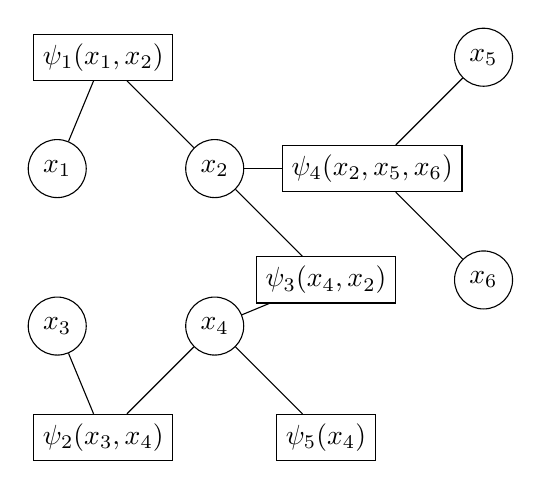
\begin{tikzpicture}[node distance=2cm]
  \node[draw, circle] (x1) {$x_1$};
  \node[draw, circle, right of=x1] (x2) {$x_2$};
  \node[draw, rectangle, right of=x2] (f4) {$\psi_4(x_2, x_5,x_6)$};
  \node[draw, circle, above right of=f4] (x5) {$x_5$};
  \node[draw, circle, below right of=f4] (x6) {$x_6$};
  \node[draw, circle, below of=x1] (x3) {$x_3$};
  \node[draw, circle, below of=x2] (x4) {$x_4$};
  \node[draw, rectangle, above left of=x2] (f1) {$\psi_1(x_1, x_2)$};
  \node[draw, rectangle, below left of=x4] (f2) {$\psi_2(x_3, x_4)$};
  \node[draw, rectangle, below right of=x4 ] (f5) {$\psi_5( x_4)$};
  \node[draw, rectangle, below right of=x2] (f3) {$\psi_3(x_4, x_2)$};
  \draw[-] (x1) -- (f1);
  \draw[-] (x2) -- (f1);
  \draw[-] (x3) -- (f2);
  \draw[-] (x4) -- (f2);
  \draw[-] (x4) -- (f3);
  \draw[-] (x2) -- (f3);
  \draw[-] (x2) -- (f4);
  \draw[-] (x4) -- (f5);
  \draw[-] (x5) -- (f4);
  \draw[-] (x6) -- (f4);
\end{tikzpicture}\]
In this example, we have six variable nodes, $x_1, x_2, x_3,x_4,x_5$ and $x_6$, and four five nodes, given by the functions $\psi_a$. The variable nodes represent the random variables in the model, and the factor nodes represent the factors that depend on these variables. The edges indicate the dependencies between the nodes. This is necessarily a bipartiate graph/.

\example{ {\bf Graph coloring}

Say that every variable takes on three different colors $x_i \in \{white,red,black\} \equiv \{0,1,2\}$. A valid coloring of a graph is such that interacting variables do not have the same color, as in this case
\[
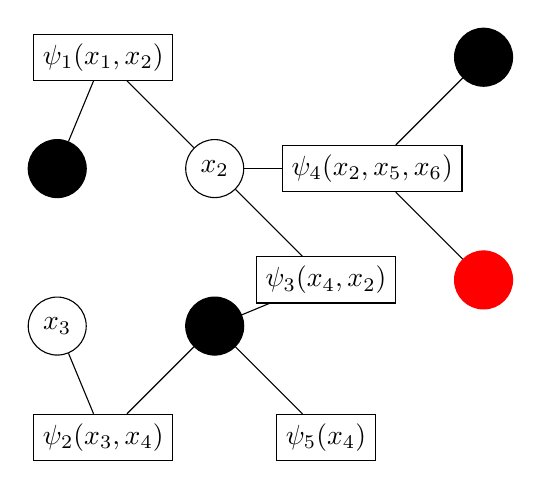
\begin{tikzpicture}[node distance=2cm]
  \node[draw, circle, fill, black] (x1) {$x_1$};
  \node[draw, circle, right of=x1] (x2) {$x_2$};
  \node[draw, rectangle, right of=x2 ] (f4) {$\psi_4(x_2, x_5,x_6)$};
  \node[draw, circle, above right of=f4, fill, black] (x5) {$x_5$};
  \node[draw, circle, below right of=f4, fill, red] (x6) {$x_6$};
  \node[draw, circle, below of=x1] (x3) {$x_3$};
  \node[draw, circle, below of=x2, fill, black] (x4) {$x_4$};
  \node[draw, rectangle, above left of=x2] (f1) {$\psi_1(x_1, x_2)$};
  \node[draw, rectangle, below left of=x4] (f2) {$\psi_2(x_3, x_4)$};
  \node[draw, rectangle, below right of=x4 ] (f5) {$\psi_5( x_4)$};
  \node[draw, rectangle, below right of=x2] (f3) {$\psi_3(x_4, x_2)$};
  \draw[-] (x1) -- (f1);
  \draw[-] (x2) -- (f1);
  \draw[-] (x3) -- (f2);
  \draw[-] (x4) -- (f2);
  \draw[-] (x4) -- (f3);
  \draw[-] (x2) -- (f3);
  \draw[-] (x2) -- (f4);
  \draw[-] (x4) -- (f5);
  \draw[-] (x5) -- (f4);
  \draw[-] (x6) -- (f4);
\end{tikzpicture}\]

How do you define a probabilistic measure that concentrates on top of valid colorings? Well, just define
\begin{eqnarray*}
\psi_{1,2,3}(x,y) &=& (1-\delta_{x,y}) \\
\psi_{4}(x,y,z) &=& (1-(1- (1-\delta_{x,y})(1-\delta_{y,z})(1-\delta_{x,z}))) \\
\psi_5(x) = 1
\end{eqnarray*}
and $P(x_1\ldots,x_6)$ will be zero in all non valid colorings, and will be $1/C$ in all $C$ valid colorings.

 Notice, {\it en passant}, that if you could compute $P(x_1,\ldots,x_6)$ you could inmediately know how many colorings there are, by just inverting any non zero value of $P(\ldots) =1 /C$.

}

The relevance of graphical model is that often they are easy to write down, meaning, it is easy to propose a meaningful set of local interactions that define your particular problem. However, the full probability disitribution is of little use, for the following reasons:
\begin{enumerate}
 \item Most of the time, you want general properities (macro states), not a microscopic description of the system
 \item Evaluation of $P(\ux)$ requieres a normalization constant, and that needs a trace over all configurations of the system, which typically is exponetially many
 \item Sometimes you care about specific variables $P_i(x_i) = \sum_{\ux \setminus x_i} P(\ux)$, that also requires an unfeasible sum.
\end{enumerate}
The first issue relates to the definition of observables in statistical mechanics, while the second relates to the partition function. The third issue is less typical of statistical mechanics, but yet, connected to the approximations we typically use to solve the first two.

%Note that the rectangular nodes represent the factor nodes, while the circular nodes represent the variable nodes.

\subsection{Supersonic intro to statistical mechanics}

In statistical mechanics, the partition function and the free energy are important quantities that describe the thermodynamic properties of a system. How does that has anything to do with inference? Well, maybe it will be clearer later, but for the time being let us say that thermodynamic porperties equals general macroscopic properties of a system, and statistical mechanics make the connection between those general properties and the details of the interactions in the system.

Consider, for instance, a graphical model as the previous one. Since the overall probability of the system is given by a product of functions, it is convenient (more on this later) to write each function as an exponential:
\[ \psi_a(\ux^a) = e^{ -\beta E_a(\ux^a) }\]
where $\ux^a  = \{x_{a_1},x_{a_2}\ldots \}$ is the set of variables that appear in the given function. In this expression $\beta$ is just a scale, and you can think of the energy $E_a(x_{\partial a})$ as a cost function. The bigger the energy of a given configuration, the less probable that configuration is.

This means that these types of models can be defined in terms of an additve energy function $E(\ux) = \sum_{a} E_a(\ux^a)$ as
\begin{equation}
 P_{B}(\ux) = \frac 1 Z e^{-\beta E(\ux)} \label{eq:boltzmann}
\end{equation}

The partition function $Z$ is a function of the scale parameter $\beta$ (equivalent to an inverse temperature), and is defined as the sum or integral over all possible states of the system, weighted by their Boltzmann factors:
\begin{equation}
    Z = \sum_{\text{states}} e^{-\beta E},
\end{equation}
For continuous systems, the sum is replaced by an integral over the phase space of the system.

% The free energy $F$ is related to the partition function by the equation
% \begin{equation}
%     F = -k_B T \ln Z,
% \end{equation}
% where $k_B$ is again the Boltzmann constant and $T$ is the temperature. The free energy is a thermodynamic potential that describes the work that can be obtained from the system, and is related to the Helmholtz free energy $A$ by
% \begin{equation}
%     F = A + PV,
% \end{equation}
% where $P$ is the pressure of the system and $V$ is its volume.

In general, the free energy can be split into two parts: the internal energy $U$, which is the average energy of the system, and the entropy $S$, which is a measure of the disorder or randomness of the system:
\begin{equation}
    F = U - \frac 1 \beta S.
\end{equation}
% The internal energy $U$ can be written as
% \begin{equation}
%     U = -\frac{\partial}{\partial \beta} \ln Z,
% \end{equation}
and the energy $U$ and entropy $S$ of a system are given as macroscopic averages
\begin{equation}
U = \sum_{\text{states}} P_B(\ux) E(\ux) \qquad    S = -\sum_{\{\ux\}} P_B(\ux) \ln P_B(\ux),
\end{equation}
where the sum runs over all configurations of the microscopic variables $\ux$, {\it i.e} all the states.

By direct substitution of eq. (\ref{eq:boltzmann}) int the definition of $F$, we can relate $F$ and $Z$ as
\[ F = - \frac 1 \beta \ln Z\]

% There is a variational way to define $F$ as well. Let us assume that $F$ can be computed with any probability distribution $q(\ux)$ not necessarily equal to $P_B(\ux)$:
% \begin{equation}
% G[q(\ux)] = U[q(\ux)] - \frac 1 \beta S[q(\ux)] \label{eq:gibbs}
% \end{equation}
% This functional is called Gibbs free energy. It is a classical result in stat-mech that the smallest value in absolute that $G[q]$ can get, is when $q\equiv P_B$, and therefore equal to $F$.


% In summary, the partition function and the free energy are key quantities in statistical mechanics that describe the thermodynamic properties of a system. The partition function is a sum or integral over all possible states of the system, and the free energy is related to the partition function by a logarithmic relationship. The free energy can be split into an internal energy and an entropy term, which describe the average energy and the disorder of the system, respectively.

\subsection{Free energy as Kullback-Leibler distance}

The Kullback-Leibler (KL) divergence, also known as the relative entropy, is a way to measure the difference between two probability distributions $p(x)$ and $q(x)$. The KL divergence is defined as:
\begin{equation}
    D_{\text{KL}}(q||p) = \int q(x) \ln \frac{q(x)}{p(x)} dx,
\end{equation}
where $q(x)$ and $p(x)$ are the two probability distributions over some variable $x$. The KL divergence measures the amount of information lost when approximating the true distribution $p(x)$ with the approximate distribution $q(x)$. It has the following properties:
\begin{enumerate}
 \item $D(q||p)$ is convex in $q(x)$;
 \item $D(q||p) \geq 0$;
 \item $D(q||p) > 0$ unless $q(x) \equiv p(x)$
\end{enumerate}
Since it is a convex non-negative quantity that is zero if and only if $q(x) = p(x)$ \footnote{ almost everywhere}, it is a good starting point to find approximations, in the sense that, the lower the KL distance, the better the approximation.

Through the glasses of statistical mechanics, the true distribution is the Botlzmann distribution (\ref{eq:boltzmann}). Simple calculations relate the KL divergence to a fundamental statistical mechanics function: the free energy. Just replace $p(\ux)$ by its Boltzmann definition
\begin{eqnarray}
    D_{\text{KL}}(q||P_{B}) &=& \sum_{\text{states}} q(x)\left( \beta E(\ux) +  \ln Z \right) \ln q(x) dx \\
    &=& \beta   \sum_{\text{states}} E(\ux) q(x) +  \sum_{\text{states}} q(x) \ln q(x)  + \ln Z \\
    &=& \beta \left( G[q(x)] + \frac 1 \beta \ln Z\right) \label{eq:DklG}
\end{eqnarray}
The functional
\begin{eqnarray*}
G[q(x)]  &=& \sum_{\text{states}} E(\ux) q(x) -  \frac {-1} \beta\sum_{\text{states}} q(x) \ln q(x)  \\
&=&  \langle E(\ux) \rangle -  \frac {1} \beta S[ q(x)]
\end{eqnarray*}
its a weighted balance between the average energy $\langle E \rangle$ and the entropy
\[S[q] \equiv - \sum_{\text{states}} q(x) \ln q(x) \]
of the distribution $q(\ux)$, called Gibbs free energy. Since when $q(\ux)\equiv P_B(\ux)$ the KL distance is zero, we get
\begin{equation}
G[P_B(\ux)] = - \frac 1 \beta \ln Z \equiv F
\end{equation}
where the latter $F$ is called free energy.

Going back to equation (\ref{eq:DklG}), it is evident that the minimun of the KL distance is found at the minimum of the Gibbs functional  $G[q(\ux)]$, since $Z$ is not a function of $q$.

{\bf Key message:  } When looking for probabilities distributions of a model:
\begin{itemize}                                     \item if you are a physicist, you minimize the Gibbs functional,
 \item if you are an information theoretician, you minimize KL divergence.
\end{itemize}

This relationship between the KL divergence and the free energy is useful in the context of computational physics and machine learning, where the KL divergence can be used as a measure of the quality of an approximate distribution compared to the true distribution. By minimizing the KL divergence, one can find the optimal approximate distribution that is closest to the true distribution, and therefore obtain a more accurate representation of the system.

\subsection{Mean field approximations}
For instance, let us say we are interested in the previous graphical model. We do not know/want to compute the exact distribution. We could search for an approximated factorized distribution
\[ q_{MF}(\ux) = \prod_{i=1}^6 p_i(x_i)\]
that resembles the most to the full unknown distribution
\[ p(\ux) = \frac 1 Z  \psi_1(x_1, x_2) \psi_2(x_3, x_4) \psi_3(x_4, x_2) \psi_4(x_2, x_5,x_6) = \frac 1 Z e^{-\beta \sum_{a=1}^6 \sum_{\ux_a} E_a(\ux_a)}\]
This results in the following Gibbs functional
\[G[q_{MF}(\ux)] = \sum_a \langle E_a(\ux_a)\rangle + \frac 1 \beta \sum_i \sum_{x_i} q_i(x_i) \ln q_i(x_i) \]
Extremization of such functional results in
\[q_i(x_i) = \frac 1 Z_i e^{-\beta \sum_{a\in \partial i} \sum_{x_j|j\neq i, j\in\partial a} E_a(\ux_a) \prod_j q_j(x_j)}\]

\subsection*{Why exponentials?}

When you first study molecular physics, or statistical mechanics, you get that weird feeling that Boltzmann distribution and Entropy are connected some how. But is not clear which comes first. Why the equilibrium distribution has to be an exponential of the energy? Is this causing the shape of the entropy function or viceversa?

I haven't set my mind on this completely, but the way I understand it is that the functional form of the entropy is the single form that has a set of properties expected from the entropy, as extensiveness, positive definite, and additive over factorized distributions. So, most probably, entropy come first, causing the Boltzmann distribution.

Besides this chicken/egg controversy, there is some hand waving argument for the need of a Boltzmann factor with an extensive energy in the exponent. Since extremes of the Gibbs functional define equilibrium, and since it is a balance between energy and entropy, well, for both magnitudes to be comparable the expected value of $E(\ux)$ has to be of the order of the expected value of $\ln q(\ux)$, meaning that $q(\ux) \sim e^{E(\ux)}$. Let me put an even more hand waving argument. Entropy is given by combinatorial terms, that grow very fast with the number of particles. Therefore, if disorder is going to have a non trivial interplay with temperature, you need to counter balance the disorder with something that grows as fast.

Only exponential of the energy makes sense. If it is not exponentiated, combinatorics always win!!


\subsection*{Mean field, details}
Actually, we neede to introduce a Lagrange multiplier to force normalizaiton of the distributions when we did the Mean Field approach. So, instead of extremizing the Gibbs free energy
\[G[q_{MF}(\ux)] = \sum_a \langle E_a(\ux_a)\rangle + \frac 1 \beta \sum_i \sum_{x_i} q_i(x_i) \ln q_i(x_i) \]
We actually need to extremize a Lagrange Function:
\[L[q_{MF},\lambda_1,\ldots,\lambda_N]  = G[q_{MF}(\ux)] -\sum_i^N \lambda_i \left(\sum_{x_i} q_i(x_1) - 1 \right)\]
Extremization of such functional results in
\[q_i(x_i) = e^{1-\lambda_i/\beta} e^{-\beta \sum_{a\in \partial i} \sum_{x_j|j\neq i, j\in\partial a} E_a(\ux_a) \prod_j q_j(x_j)}\]
The extremization over the Lagrange multipliers enforces the condition, so $\lambda_i$ will take the requiered value for $q_i(x_i)$ to be normalized.

\section{Beyond Mean Field: Belief Propagation}

Mean field is quite poor. Essentially it loses all correlations in the system. We can do better, specially in trees. Lets see how.

By the way in which our graphical models are constructed, each factor node corresponds to a proability distribution of a group of variables in the absence of others, so independently, we have:
\[\forall_a p_a(\ux_a) = \frac 1 z_a e^{-\beta E_a(\ux_a)}\]
Can we build our full probability out of these factor probabilities? Yes indeed!

\subsubsection*{Bayes rule}

As you shall remember from your probability course, the conditional probability is defined as
\[P(A|B) = \frac{P(A,B)}{P(B)}\]
and is understood as the probability of having $A$ given that $B$ occurred.

So, if you have two sets of variables, that have a non null intersection, you can always write
\[ p(\ux_{a\cup b}) = p(\ux_a | \ux_b) p(\ux_b)\]
for the joint probability. Furthermore, you can write
\[ p(\ux_{a\cup b}) =  \frac { p(\ux_a ) p(\ux_b)}{p(\ux_{a\cap b})}\]

So you can iteratively merge you rentire graph (as long as it is a tree) in order to write
\begin{equation}
 P(\ux) = \prod_{a} p_a(x_a) \prod_{a \cap b\neq \varnothing} \frac 1 {p(\ux_{a\cap b})}
\end{equation}
This is cool, since we have a new family of possible distributions to use as a test in Gibbs-KL minimization!!

Let us assume, for notation simplicity, that intersections between factors nodes happen always at a single varialbe, as is the case in the graphical model
\[
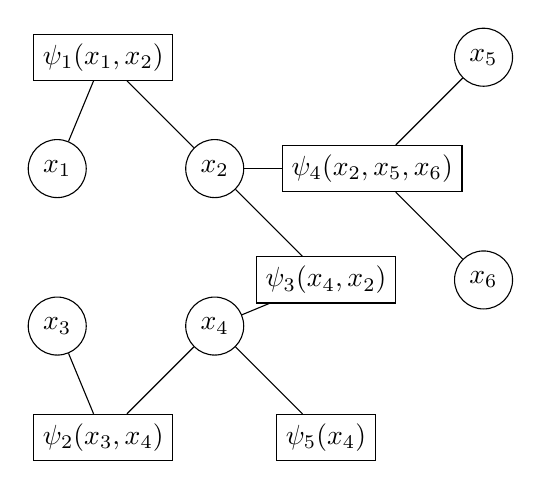
\begin{tikzpicture}[node distance=2cm]
  \node[draw, circle] (x1) {$x_1$};
  \node[draw, circle, right of=x1] (x2) {$x_2$};
  \node[draw, rectangle, right of=x2] (f4) {$\psi_4(x_2, x_5,x_6)$};
  \node[draw, circle, above right of=f4] (x5) {$x_5$};
  \node[draw, circle, below right of=f4] (x6) {$x_6$};
  \node[draw, circle, below of=x1] (x3) {$x_3$};
  \node[draw, circle, below of=x2] (x4) {$x_4$};
  \node[draw, rectangle, above left of=x2] (f1) {$\psi_1(x_1, x_2)$};
  \node[draw, rectangle, below left of=x4] (f2) {$\psi_2(x_3, x_4)$};
  \node[draw, rectangle, below right of=x4] (f5) {$\psi_5( x_4)$};
  \node[draw, rectangle, below right of=x2] (f3) {$\psi_3(x_4, x_2)$};
  \draw[-] (x1) -- (f1);
  \draw[-] (x2) -- (f1);
  \draw[-] (x3) -- (f2);
  \draw[-] (x4) -- (f2);
  \draw[-] (x4) -- (f3);
  \draw[-] (x2) -- (f3);
  \draw[-] (x2) -- (f4);
  \draw[-] (x4) -- (f5);
  \draw[-] (x5) -- (f4);
  \draw[-] (x6) -- (f4);
\end{tikzpicture}\]
where, for instance $\ux_{1\cap 3} = x_2 = \ux_{1\cap 4}$. Since the same set of variables $\ux_{a\cap b}$ can arrise from different $a$'s and $b$'s, it si more commonly written
\begin{equation}
 P(\ux) = \prod_{a} p_a(\ux_a) \prod_{i} \frac 1 {p_i(x_i)^{d_i-1}} \label{eq:BPprob}
\end{equation}
where $d_i$ is the degree of variable $i$.

\subsubsection{Bethe free energy}

Notice that any graphical model, not necessarily a tree, is subsceptible of being approximated this way. In the case of trees, it is an exact representation of the probability, while in the rest of graphs, it is an approximation. To mark the ide that it not necessarily is exact, we call the local probability distributions as beliefs and replace $p_a(\ux_a) \to b_a(\ux_a)$.

If we replace the family (\ref{eq:BPprob}) into the Gibbs free energy, we get the so called Bethe free energy is
\begin{equation}
 G_{BP}[\{b_R(\bm{s}_R)\}]  = \sum_{a} G_a[b_{a}(\ux_a)] + \sum_i (1-d_i) G_i[b_i(x_i)] \label{eq:free_en_Bethe_D}
\end{equation}
where $d_i$ is the number of factors (functions $\psi_a$) that the $i$-th variable belongs to.

The distributions $b_a(\ux_a)$ and $b_i(x_i)$ are the variables over which we minimize the free energy functional, and should approximate the marginals of the Boltzmann. For this reason, the functional minimization is not done considering the independent functions $b(\ux)$, but they are linked by the marginalization condition \index{Boltzmann distribution}
\begin{equation}
\forall_a \forall_{i\in a} \:\: b_i(x_i) = \sum_{\ux_{a \setminus i}} b_a(\ux_a). \label{eq:marginalizacion_bethe}
\end{equation}

\subsubsection*{Constrained minimization}
This relations can easily be enforced with a set of Lagrange multipliers, as we reminded you at the beginning. The Lagrange functional is
\[ L[\{b_R(\bm{s}_R), \{m_{a,i}(x_i)\}\}]  = G_{BP}[\{b_R(\bm{s}_R)\}] +  \sum_{a} \sum_{i \in a} \sum_{x_i} m_{a,i}(x_i) \left( b_i(x_i) - \sum_{\ux_{a \setminus i}} b_a(\ux_a)]  \right)\]

Extremizaiton of the Lagrange function produces the following relations
\begin{eqnarray}
 b_a(\ux_a) &=& \frac 1 z_a e^{-\beta E_a(\ux_a) }\prod_{j\in a} \prod_{b \in \partial j \setminus a} m_{b,j}(x_j) \label{eq:ba} \\
 b_i(\ux_i) &=& \frac 1 z_i e^{-\beta E_i(x_i) } \prod_{b \in \partial i} m_{b,i}(x_i) \label{eq:bi}
\end{eqnarray}
relating the local porbability distributions to the values of the local energy and the lagrange multipliers $m_{a,i}(x_i)$.

\subsubsection*{Message Passing equations}
As usual, extremization with respect to the Lagrange multipliers reproduces the constraints they are enforcing, namely eq. (\ref{eq:marginalizacion_bethe}). After writing this conditions in terms of eqs. (\ref{eq:ba,eq:bi}), we get the following relation among Lagrange multipliers:
\begin{equation}
 m_{a\to i}(x_i) = \sum_{\ux_{a \setminus i}} \frac 1 z_a e^{-\beta (E_a(\ux_a) )}\prod_{j\in a \setminus i} \prod_{b \in \partial j \setminus a} m_{b,j}(x_j)
\end{equation}

usually understood as {\bf message passing} equations.
%From now on, we will refer to a Bethe graph as a random regular graph. Like any regular graph, each node has the same connectivity $\forall_i \: d_i \equiv d$, and the random character implies that the size of the cycles grows as $\log N$. The fundamental property of a Bethe graph is that the local structure is in the form of a tree (there are no short cycles when $N\to \infty$), and this allows us to use the Bethe approximation with confidence and generally with good results \cite{cowell_bethe_exact_tree}. \index{Bethe graph}

While the approximation is exact in a tree, and is very good in a graphs with large loops, in systems with short cycles the results are usually much worse.


\subsection{A simple example: coloring trees}
Let us go back to the  {\bf Graph coloring} example. We already with this functions
\begin{eqnarray*}
\psi_{1,2,3}(x,y) &=& (1-\delta_{x,y}) \\
\psi_{4}(x,y,z) &=& (1-(1- (1-\delta_{x,y})(1-\delta_{y,z})(1-\delta_{x,z}))) \\
\psi_5(x) = 1
\end{eqnarray*}
 the probability measure
\[ P(x_1\ldots,x_6) \propto  \psi_1(x_1, x_2) \psi_2(x_3, x_4) \psi_3(x_4, x_2) \psi_4(x_2, x_5,x_6) \psi_5(x_4)\]
concentrates only on the  valid colorings.

But, this measure doesn't look as we the exponential of an energy, since the $\psi_a(\cdot)$ functions aren't equivalent to exponentials of local interactions. First, this si, in itself not a problem. Although we wrote the BP equations in the physical way, we can directly replace the energy by the functions $\psi_a$, as in \begin{equation}
 m_{a\to i}(x_i) = \sum_{\ux_{a \setminus i}} \: \psi_a(\ux_a) \: \prod_{j\in a \setminus i} \prod_{b \in \partial j \setminus a} m_{b,j}(x_j)
\end{equation}

But still, you might want not to do that. In that case, you can define
\begin{eqnarray*}
E_{1,2,3}(x,y) &=& \delta_{x,y} \\
E_{4}(x,y,z) &=& \delta_{x,y} +  \delta_{y,z} + \delta_{x,z} \\
E_5(x) = 0
\end{eqnarray*}
and use a high value of $\beta$ in your algorithm.  The energy terms now are zero for valid local configurations of colors, and 1 for invalid ones. Since $\beta$ is big, the exponentials
\[ e^{-\beta \psi_a(\cdot)} = \left\{ \begin{array}{ll}
1 & \mbox{ coloring is valid } \\
e^{-\beta} \ll 1 & \mbox{ coloring is invalid }
\end{array} \right.
\]
which for practical purposes is equivalent to the hard constraint definition.



\subsection{A clever way to count}

In particular in the tree coloring problem above, message passing equations are completely trivial, since there is no bias towards any particular color, all messages turn out to be flat
\[ m_{a\to i} (x_i) = (\frac 1 3,\frac 1 3,\frac 1 3)\]
for the case of three-colors.

Yet, there are two possible ways in which we could use the BP solution. First, we could compute the entropy
\[S = \sum_{a} S[b_a(\ux_a)]+ \sum_i (1-d_i) \sum_{x_i} S[b_i(x_i)] \qquad \mbox{where } S[b] =  -\sum_{x} b(x) \ln b(x)\]

If you evaluate in this case, you get $S=\ln 48.0$, which coincide with the 48 valid configurations, and the fact that the entropy of an uniform distribution is the log of the number of states.

You could also repeat the message passing and the entropy calculation, but forcing one node, let's say $x_4$ to have a particular color. You can do that by simply changing $\psi_5$:
\[\psi_5(x) = (1,0,0) \]
In that case, you get $S = \ln 16$, again consistent with the number of valid configurations.

\section{The zero patient problem}

{\Large \bf Note:} this is an extraction of the paper :

F. Altarelli. et. al., ``Bayesian Inference of Epidemics on Networks via Belief Propagation, '', Phys. Rev. Lett. 112, 118701 --Published 17 March 2014


\paragraph*{The SIR model on graphs \label{sec:The-SIR-model-on-graphs}}

The susceptible-infected-recovered (SIR) model of spreading is a stochastic dynamical model in discrete time defined over a graph $G=(V,E)$. At time $t$ a node $i$ can be in one of three states (\emph{infected}, \emph{suceptible} or \emph{recovered}) represented by a variable $x_{i}^{t}\in\left\{ S,I,R\right\} $.
% We assume defined known \emph{transmission probabilities} $p_{ij}\in\left[0,1\right]$ associated to each directed edge $(ij)\in E$ and a recovery probability $r_{i}\in\left[0,1\right]$ associated with each node $i$. The dynamical process is defined as follows: at each time step $t$, each node $i$ in the infected state, $x_{i}^{t}=I$ attempts contagion to susceptible neighbors in $\left\{ j\in\partial i:x_{j}^{t}=S\right\}$, each will succeed with independent probability $p_{ij}$, bringing $x_{j}^{t+1}=I$. Afterwards, node $i$ will attempt recovery with probability $r_{i}$, which if successful will bring $x_{i}^{t+1}=R$. All nodes for which none of these events succeeded conserve their prior state, i.e. $x_{k}^{t+1}=x_{k}^{t}$.
The dynamical process is defined as follows: at each time step $t$, each node $i$ in the infected state attempts to infect each one of its susceptible neighbors $\left\{ j\in\partial i:x_{j}^{t}=S\right\}$, succeeding with independent probabilities $p_{ij}\in\left]0,1\right]$ (which we assume known); then, node $i$ attempts to recover, succeeding with probability $r_{i}\in\left[0,1\right]$ (also assumed known).
The dynamics is clearly irreversible, as a given node can only undergo the transitions $S\to I\to R$, and thus a stationary condition will be reached in finite time (with all nodes either in the $S$ or $R$ state provided $r_{i}>0$).
Two important special cases of SIR are: \textbf{(a)} the Independent Cascade (IC) model, obtained when $r_{i}\equiv1$, which has been extensively studied in the related context of optimization of the spread of information \cite{kempe_maximizing_2003} and a particular sub-case of which is {\em bootstrap percolation} with threshold $\theta = 1$ (obtained when $p_{ij}\equiv 1$);
\textbf{(b)} the susceptible-infected (SI) model, obtained when $r_{i}\equiv0$. It should be noted that the IC model describes completely the SIR model for arbitrary $r_{i}$ in the infinite time limit, while the infinite time limit of the SI model is rather trivial, as all nodes in the connected component of an initially infected node will be infected at time $t\to\infty$. Nevertheless, the evolution in time can show rich and interesting characteristics.
%\begin{figure}
%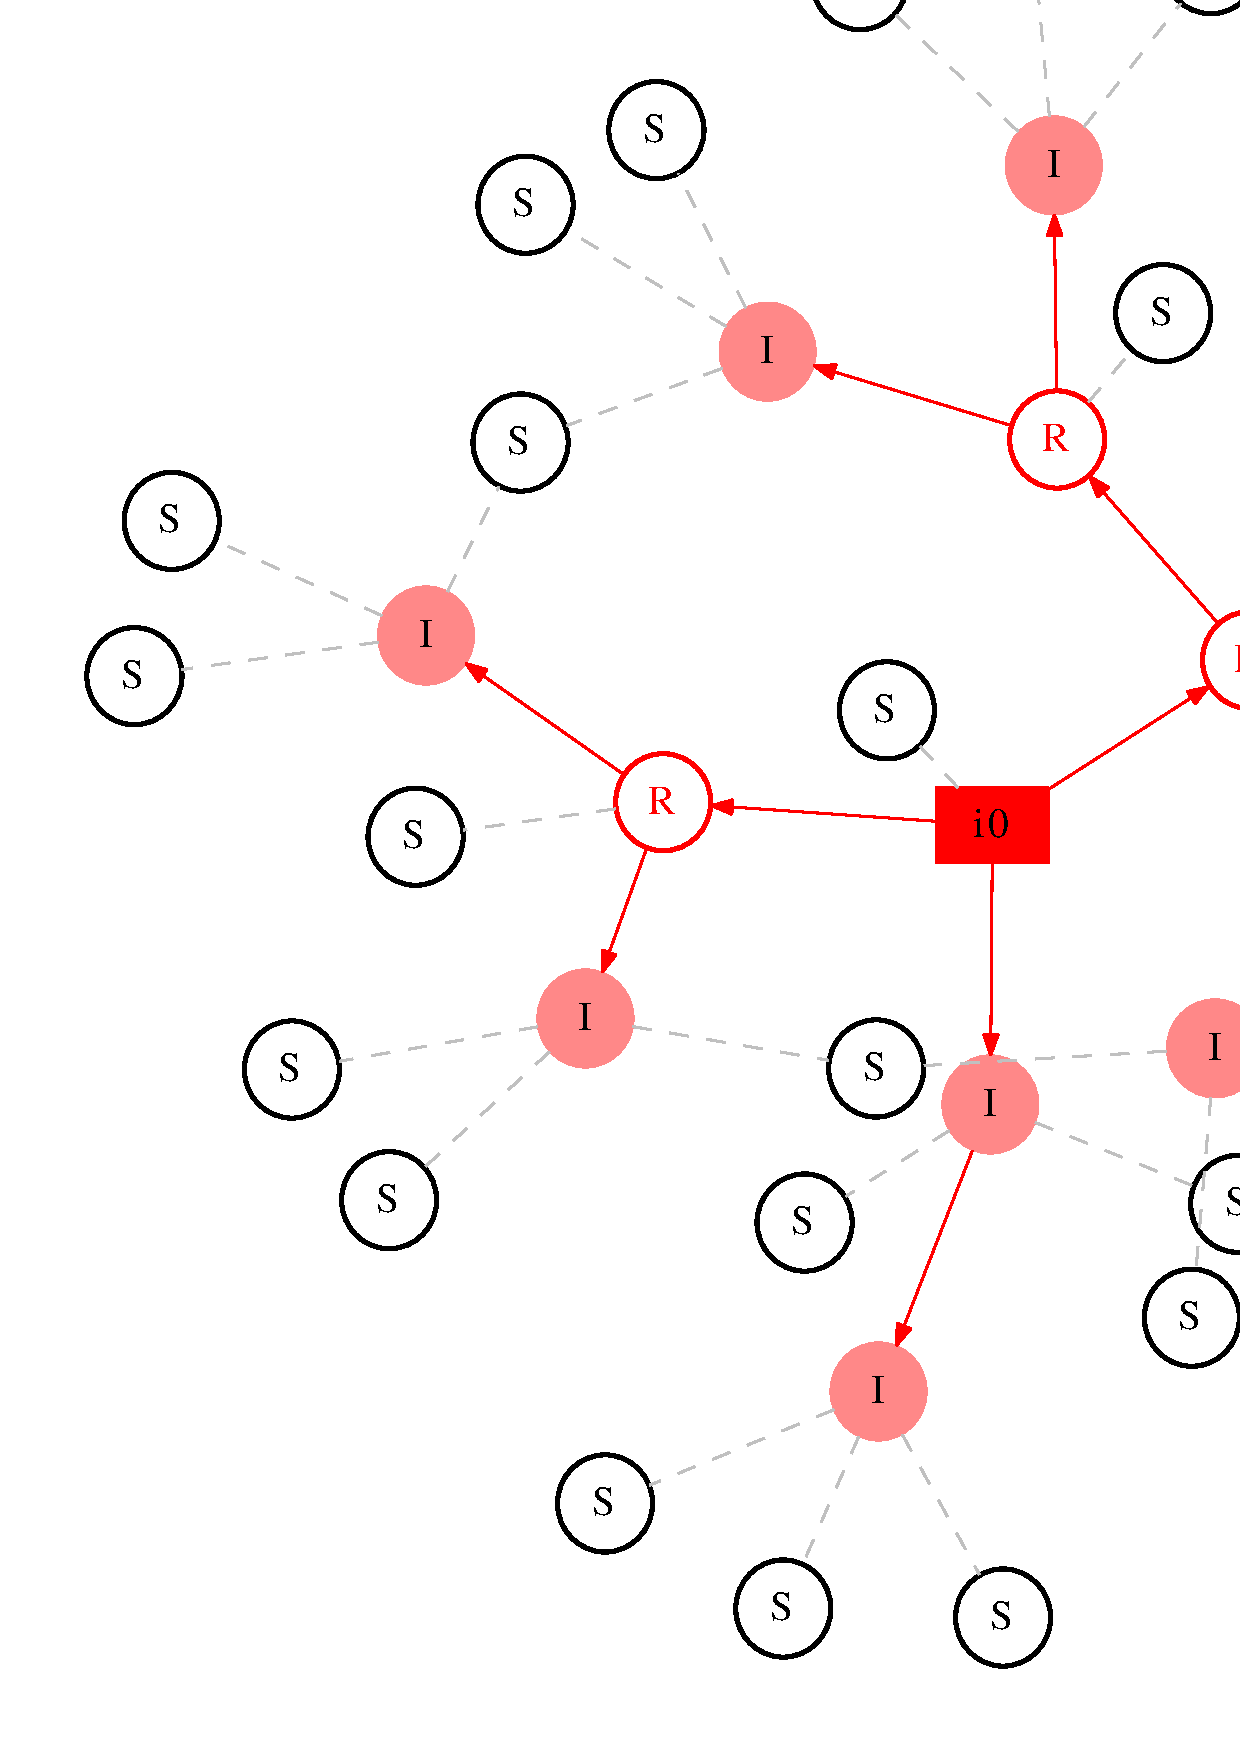
\includegraphics[width=0.65\columnwidth, angle=0]{zero_patient/epidemy}
%\caption{\label{fig:epidemy} Example of the snapshot of an epidemy after $T=3$ time
%steps. The zero patient corresponds to the square node.}
%\end{figure}


\paragraph*{Self-consistent equations for spread computation.}

Assume that a certain set of nodes starts the infection at time $t=0$,
i.e. with $x_{i}^{0}=I$. The SIR model can be re-stated as following: recovery times $g_{i}$ and {\em delay parameters} $s_{ij}$ are drawn
respectively from $\mathcal{G}_{i}\left(g_{i}\right)=r_{i}\left(1-r_{i}\right)^{g_{i}}$
and $\omega_{ij}\left(s_{ij}|g_{i}\right)=p_{ij}\left(1-p_{ij}\right)^{s_{ij}}$ for $s_{ij}\leq g_i$ and $\omega_{ij}\left(\infty|g_i\right)=\sum_{s>g_i}p_{ij}\left(1-p_{ij}\right)^{s}$;
i.e. the recovery time follows a geometric distribution and the delay
in transmission follows a geometric distribution truncated by $g_{i}$.
Afterwards, the infection times $t_{i}$ can be computed deterministically
as the ones satisfying $1=\phi_{i}=\delta\left(t_{i},\1\left[x_{i}^{0}\neq I\right]\left(\min_{j\in\partial i}\left\{ t_{j}+s_{ji}\right\} +1\right)\right)$
for every $i$. This representation makes it possible to write the
distribution of infection and recovery times $\mathbf{t},\mathbf{g}$
given the initial state $\mathcal{P}\left(\mathbf{t},\mathbf{g}|\mathbf{x}^{0}\right)=\sum_{\mathbf{s}}\mathcal{P}\left(\mathbf{s}|\mathbf{g}\right)\mathcal{P}\left(\mathbf{t}|\mathbf{x}^{0},\mathbf{g},\mathbf{s}\right)\mathcal{P\left(\mathbf{g}\right)}$
giving

\begin{eqnarray}
\mathcal{P}\left(\mathbf{t},\mathbf{g}|\mathbf{x}^{0}\right) & = & \sum_{\mathbf{s}}\prod_{i,j}\omega_{ij}\prod_{i}\phi_{i}\mathcal{G}_{i}
	\label{eq:direct}
\end{eqnarray}



\paragraph*{Bayesian inference in the SIR model}

Assume to know the sate of an epidemics at time $t=T$, i.e. the state
of every node $x_{i}^{T}\in\left\{ S,I,R\right\} $ but to possess
only probabilistic prior information about the set of initially infected
nodes; specifically, assume that nodes are initially infected with i.i.d. {\em a priori} probability $\mathcal{P}\left(\mathbf{x}^{0}\right)=\prod_{i}\gamma_{i}\left(x_{i}^{0}\right)$.
Starting with $\mathcal{P}\left(\mathbf{x}^{T}|\mathbf{t},\mathbf{g}\right)=\prod_{i}\xi_{i}\left(t_{i},g_{i},x_{i}^{T}\right)$
where $\mathcal{\xi}_{i}=\1\left[x_{i}^{T}=I,t_{i}\leq T<t_{i}+g_{i}\right]+\1\left[x_{i}^{T}=S,t_i < T\right]+\1\left[x_{i}^{T}=R,t_{i}+g_{i}\leq T\right]$,
the posterior distribution $\mathcal{P}\left(\mathbf{x}^{0}|\mathbf{x}^{T}\right)\propto\sum_{\mathbf{t,g}}\mathcal{P}\left(\mathbf{x}^{T}|\mathbf{t},\mathbf{g}\right)\mathcal{P}\left(\mathbf{t},\mathbf{g}|\mathbf{x}^{0}\right)\mathcal{P}\left(\mathbf{x}^{0}\right)$
can be expressed thanks to \eqref{eq:direct} as
\begin{equation}
\mathcal{P}\left(\mathbf{x}^{0}|\mathbf{x}^{T}\right)\propto\sum_{\mathbf{t},\mathbf{g},\mathbf{s}}\prod_{i,j}\omega_{ij}\prod_{i}\phi_{i}\mathcal{G}_{i}\gamma_{i}\xi_{i}\label{eq:Bayes}
\end{equation}



\paragraph*{Belief Propagation equations for the likelihood function}

For the derivation of the Belief Propagation (BP) equations we will rewrite \eqref{eq:Bayes} by introducing $t_{j}'=t_{j}+s_{ji}$.
Define $\phi_{ij}=\omega_{ij}\left(t'_{i}-t_{i}|g_{i}\right)\omega_{ji}\left(t'_{j}-t_{j}|g_{j}\right)$
and $\phi_{i}=\delta\left(t_{i};\1\left[x_{i}^{0}\neq I\right]\left(\min_{j\in\partial i}\left\{ t'_{j}\right\} +1\right)\right)$;
then
\[\mathcal{P}\left(\mathbf{x}^{0}|\mathbf{x}^{T}\right)\propto\sum_{\mathbf{t},\mathbf{t}',\mathbf{g}}\prod_{i<j}\phi_{ij}\prod_{i}\phi_{i}\mathcal{G}_{i}\gamma_{i}\xi_{i}.\]
In particular, one can recover a factor graph topology equivalent to the one of the original
graph of contacts (as in \cite{altarelli_optimizing_2012,*altarelli_large_2013})
by adding dynamical variables defined by triplets $(g_{i}^{(j)},t_{i}^{(j)},t'_{j})$
and regrouping terms $\psi_{i}=\phi_{i}(t_{i},\mathbf{t}'_{\partial i})\prod_{j\in\partial i}\delta(t_{i}^{(j)},t_{i})\delta(g_{i}^{(j)},g_{i})$ (See Figs.~\ref{fig:fg}c,\ref{fig:fg}d).
We obtain the effective model
\begin{equation}
\mathcal{Q}\propto\prod_{i<j}\phi_{ij}\prod_{i}\psi_{i}\mathcal{G}_{i}\gamma_{i}\xi_{i}
\label{eq:effective}
\end{equation}
in terms of which $\mathcal{P}\left(\mathbf{x}^{0}|\mathbf{x}^{T}\right)\propto\sum_{\mathbf{t},\mathbf{t}',\mathbf{g}}\mathcal{Q}\left(\mathbf{g},\mathbf{t},\mathbf{t}',\mathbf{x}^{0}\right)$.
\begin{figure}
\includegraphics[width=1.0\columnwidth]{zero_patient/fgsir}
\caption{Factor graph representations for irreversible dynamics\label{fig:fg}. (a) Original graph (b) Loopy, naive factor graph for an irreversible deterministic dynamics (c) Dual tree factor graph (d) Factor graph for the SIR model given in \eqref{eq:effective} with known epidemy age (e) Factor graph representation with unknown epidemy age.}
\end{figure}

Belief propagation equations can be written for the efficient approximate computation of marginals of \eqref{eq:effective} (See SM). The BP update of $\psi_{i}$ can be computed in time $O\left(G\cdot T\cdot\left|\partial i\right|\right)$, where $G$ is the maximum allowed recovery delay,
and the one of $\phi_{ij}$ in time $O\left(G^{2}\cdot T\right)$. In practice, $G$ can be taken constant for a geometric distribution $\mathcal G$.
A single BP iteration can be thus computed in time $O\left(T\cdot G^{2}\cdot\left|E\right|\right)$. We remark that the BP equations for the posterior distribution are exact (and have a unique solution) on tree factor graphs \cite{pearl_reverend_1982}. As the topology of the factor graph mirrors the one of the original graph, \eqref{eq:effective} allows the exact computation of posterior marginals for the SIR model on tree graphs (at difference with the DMP method).

\paragraph*{Unknown epidemy age}
The start time of the epidemy was assumed up to now to be known, but this may be unrealistic. Coping with the case of unknown initial time is easy; starting with an upper bound on the epidemic duration, it suffices to consider the dynamical process to start from the all-susceptible state but to allow nodes to be spontaneously infected at an arbitrary time with (small) uniform probability. This is equivalent to the addition of a fictitious virtual neighbor to every node with no constraint in its activation time besides the prior probability $\varepsilon_i(g''_i,t''_i,t_i)=\delta(t''_i,\infty)(1-2\gamma)+\gamma$ of spontaneous infection (See Fig.~\ref{fig:fg}e).%The case of known epidemy age, with a single epidemic origin, is recovered by considering the self-infection probability to be zero for times different from the initial one.

\paragraph*{Identification of a single source}
Through out the rest of the paper we restrict ourselves to random regular graphs of degree $k=4$ and $N=1000$ nodes with homogeneous propagation probability $p_{ij}\equiv p$ and recovery probability $r_i\equiv r$ in order to make comparison with other inference methods simpler. An example of inference for an epidemy with recovery and transmission probabilities $\lambda=\mu=0.5$ is depicted in Fig.~\ref{fig:infertimes}. For each node, an infection time distribution is computed as a BP marginal and the mean and standard deviation of this ditribution are plotted against the true time.
We compared the inference performance of BP with the one of DMP in the case of a single epidemic source. The DMP method iterates the forward probabilistic transmission equations of \cite{karrer_message_2010} to obtain single-site trajectory probability distributions. Afterwards, using a single-site factorization hypothesis for joint distribution at the observation time, it gives a simple factorized expression of the likelihood of the observed epidemy. DMP is shown \cite{lokhov_inferring_2013} to outperform other more classical estimations of the epidemy origin \cite{shah_detecting_2010,*shah_rumors_2011,comin_identifying_2011}.
%In figure \ref{fig:rank_vs_lambda_T6_mu1} and \ref{fig:rank_vs_lambda_T11_mu05} we show the average normalized ranking of BP, DMP and Jordan centrality \cite{shah_detecting_2010,shah_rumors_2011,comin_identifying_2011} estimations. For small observations times ($T=5$ in figure \ref{fig:rank_vs_lambda_T6_mu1}) BP is slightly more accurate than DMP. Note that for short times the epidemy structure is particularly simple on expander graphs. For bigger epidemies BP substantially outperforms DMP in terms of accuracy, in some cases outstandingly (see Fig.~\ref{fig:rank_vs_lambda_T11_mu05}).
\begin{figure}
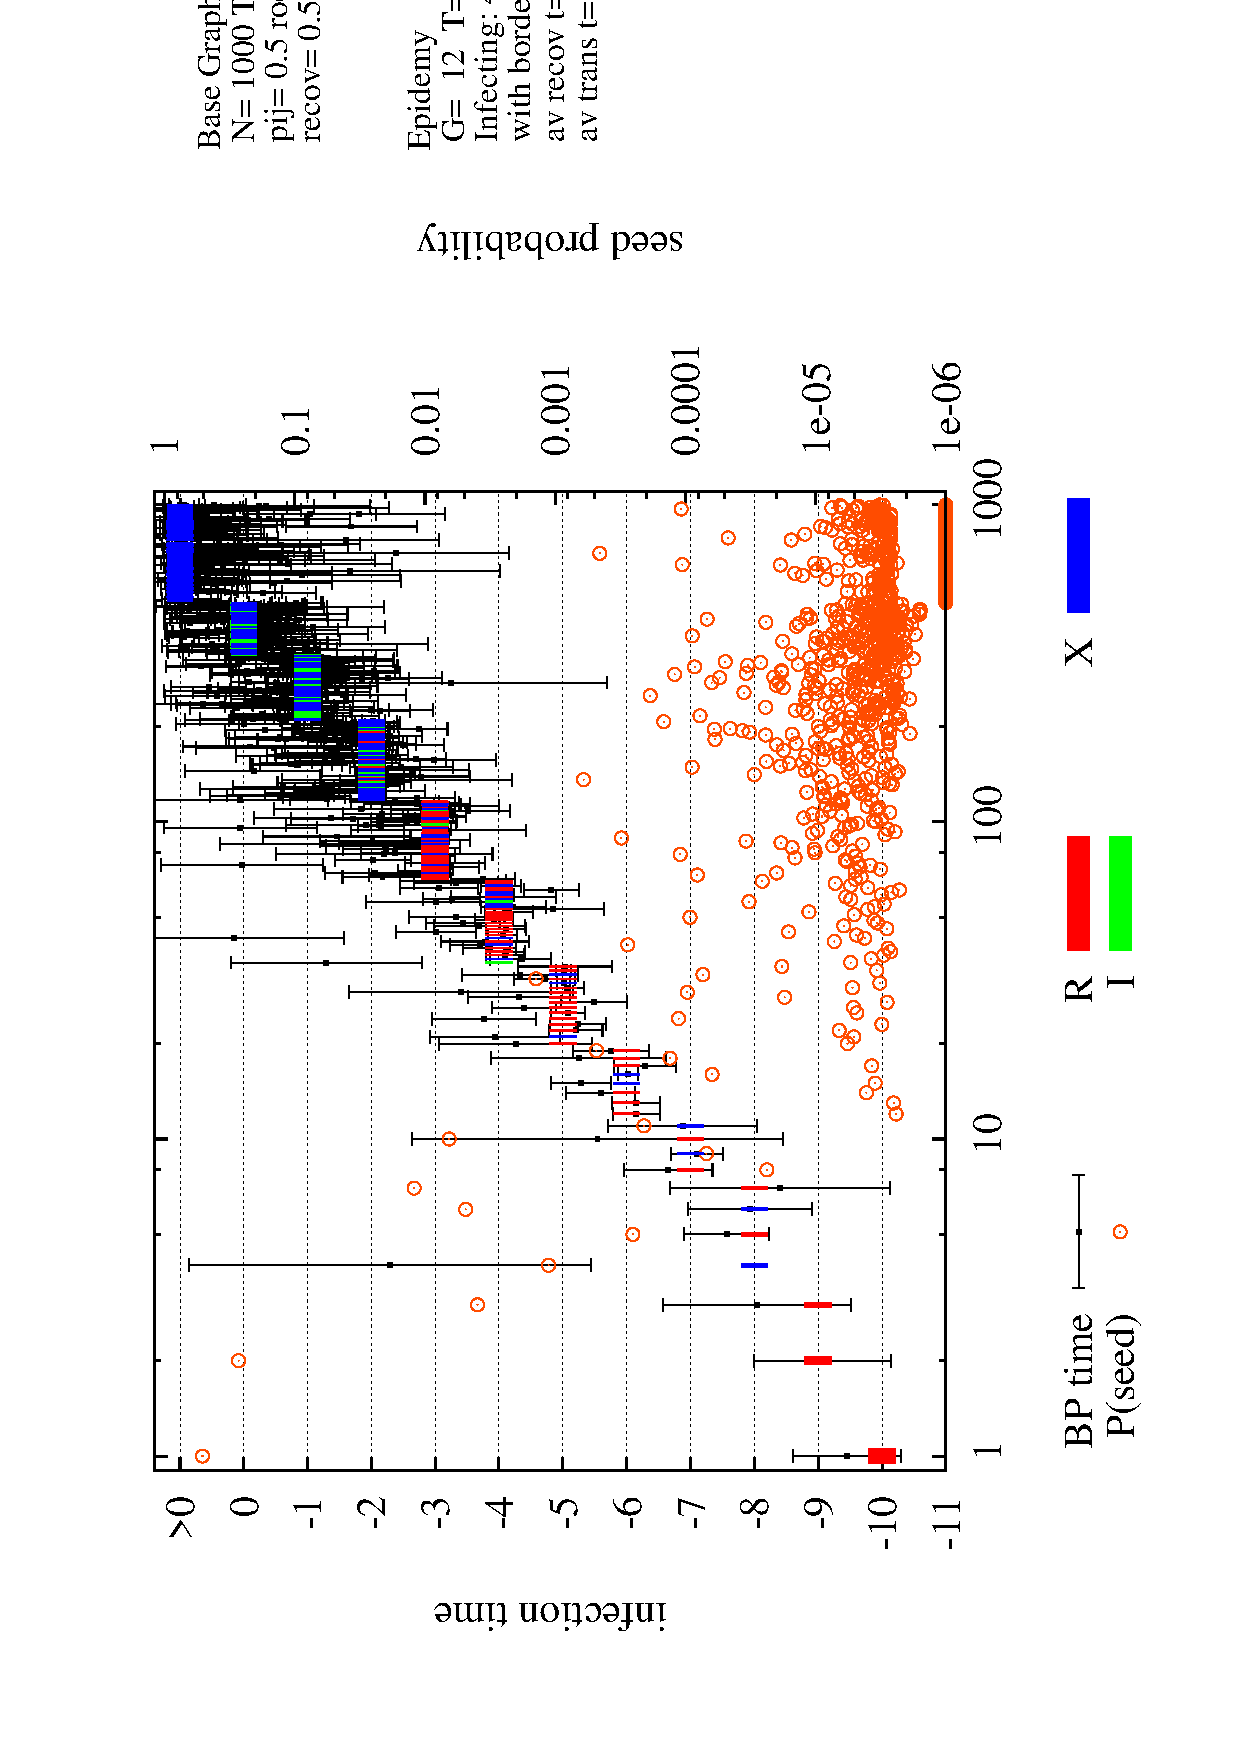
\includegraphics[height=1.0\columnwidth, angle=270]{zero_patient/infertimes}
\caption{(Color online) An example of inference on a RRG with $N=1000,k=4$, with $\lambda=\mu=0.5$ and prior seed probability $10^{-6}$, and observations at time $T=0$ on $\xi=0.7$ of the nodes on an epidemy with $t_0=-10$. Each point in the x axis corresponds to a vertex on the graph. Nodes are ordered by their real infection time (blocks, R=recovered, I=infected and X=unknown). The mean and standard deviation of their BP posterior marginal distribution of infection time is plotted (black dots and error bars) along with the marginal posterior probability of self-infection (orange, circles, right axis).\label{fig:infertimes} }
\end{figure}

Two methods are used as benchmarks: Jordan centrality \cite{shah_detecting_2010,shah_rumors_2011,comin_identifying_2011} and DMP. In figure \ref{fig:rank_vs_lambda_T11_mu05} we show the average normalized rank given to the true zero patient by BP, DMP and Jordan centrality over $10^3$ instances with observation time $T=10$ and recovery probability $\mu=0.5$. Since DMP requires a defined value of the observation time, we here assume that $T=10$ is known for both DMP and BP. It is seen how BP outperforms DMP by a large margin in the probability of finding the epidemy origin. The inset shows also a remarkable difference in the normalized ranking of the true origin given by all three algorithms, again BP outperforming the other two.
%For small observations times ($T=5$ in figure  \ref{fig:rank_vs_lambda_T6_mu1}) BP is slightly more accurate than DMP. Note that short times the epidemy structure is particularly simple on expander graphs. For bigger epidemies BP substantially outperforms DMP in terms of accuracy, in some cases outstandingly (see Fig. \ref{fig:rank_vs_lambda_T11_mu05}).


%DA RIVEDERE IN BASE AI RISULTATI: As in any belief propagation approach, we rely upon convergence to get an estimate of the desired quantities. When epidemy sizes grow (see purple dotted line) the message passing heuristic begin failing to converge within 300 iteration steps. After examining not convergent samples we decided to use the information from BP even when convergence is not reached. It can be seen in Fig. \ref{fig:rank_vs_lambda_T11_mu05} that in this regime the predictions obtained are worse than those obtained with DMP, but still better than Jordan centrality, and better than a random estimation.

%\begin{figure}
%\includegraphics[width=0.65\columnwidth, angle=270]{zero_patient/T6_rank_vs_lambda_mu1.eps}
%\caption{\label{fig:rank_vs_lambda_T6_mu1} }
%\end{figure}


\begin{figure}
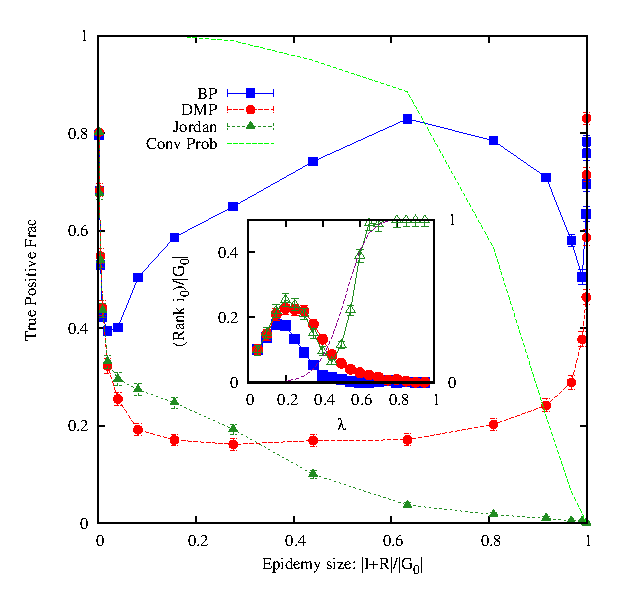
\includegraphics[width=1\columnwidth, angle=0]{zero_patient/T11_rank_vs_lambda_mu05}
\caption{\label{fig:rank_vs_lambda_T11_mu05} Normalized rank given to the true zero patient by Jordan, DMP and BP methods, as a function of the transmission probability $\lambda$, averaged over $10^3$ instances of $N=1000, k=4$ RRG with observation time $T=10$. Most relevant part is $0.2<\lambda<0.8$ where the epidemy size (purple, right axis) spans most of its range. For too large epidemies BP has convergence problems (green, right axis), nevertheless some relevant information is still present in the (unconverged) marginals. The inner plot shows the probability of finding the true origin of the epidemy using DMP and BP as a function of the average epidemy size for each value of $\lambda$.}
\end{figure}



\paragraph*{Incomplete information}

In a more realistic setup, the state of many nodes in the population is usually not known. Calling $\xi$ the fraction of unobserved sites (denoted in state $X$), we test the average ranking given to the real zero patient by BP, and compared it with other three methods in Fig.~\ref{fig:rank_vs_obs}. We found that DMP can be improved over its original presentation if the dyamics MP equations are not iterated over all the nodes of the graph, but only over the connected component of $I,R$ and $X$ nodes. We refer to this version as DMP-restricted or DMPr (see SM for details). Jordan centrality is also computed over this connected component as in \cite{lokhov_inferring_2013}. BP is quite efficient in this regime, finding the true zero patient in more than $75\%$ of instances up to $60\%$ of unobserved sites (inner plot), and outperforming all other methods for almost all $\xi$.% and \ref{fig:perfect_inf}.

\begin{figure}
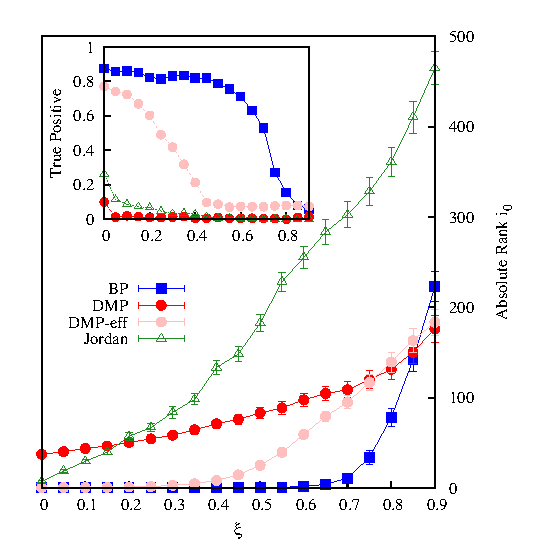
\includegraphics[width=1\columnwidth, angle=0]{zero_patient/T11_rank_vs_obs}
\caption{\label{fig:rank_vs_obs} }
\end{figure}

\begin{figure}
\includegraphics[width=1\columnwidth, angle=0]{zero_patient/multiseeds}
\caption{Inference of multiple seeds with $r=1,p_{ij}=0.5$, seed probability $0.002$ and variable $T-t_0$ (unknown to the inference algorithm). Inference was attempted for each of 1 000 instances for every $T-t_0$, and the the sum of the rankings of the true seeds in the outcome order is plotted vs. the true number of seeds. Inset: the average area of the ROC curve. Each ROC curve was computed restricted to the epidemic subgraph.\label{fig:multiseeds} }
\end{figure}
\paragraph*{Inference of multiple sources}
If the origin of the epidemics is not a single source, but a set of sources, methods based on the exhaustive exploration of initial states like DMP suffer a combinatorial explosion. This problem does not affect BP, as the trace over initial conditions is performed directly within the framework. We show in Fig.~\ref{fig:multiseeds} experiments with multiple seeds, showing that effective inference can also be achieved in this regime.

\paragraph*{Dynamically evolving networks}
We studied the case of dynamically evolving networks, in which the transmission probility $p_{ij}$ depends on time (representing the time-evolution of interactions between agents). For this purpose, we employed the interesting dataset \cite{isella_whats_2011}, corresponding to a large list of time-stamped face-to-face contacts between couples of visitors in a cultural event. We aggregate the 20 second resolution of the data into $T$ effective time steps, and simulate the progression of a virtual epidemy initiated by a random visitor. We employed the following set of parameters: probability $p^{20s}_{ij}=0.1$ of contagion in a 20 second interval, recovery probability $r=0.1$, and $T-t_0=30$. We employed the last four days of the event, in which the volume of visitors was larger, and simulated 2000 random propagations. We kept the 50 epidemies with larger number of infected individuals ($98\pm 14$). The correct origin was identified perfectly in 13 cases (26\%), and in general its normalized ranking was in average $0.07\pm0.11$. Finally, also infection times were recovered with good accuracy: the probability assigned to the correct infection time (for infected individuals) was in average $0.53\pm 0.06$, and the average absolute error in the infered infection time was $0.76\pm 0.23$.

%\paragraph*{Conclusions}

%A more general formulation that includes recovery probabilities $r_{i}$ that depend on the time after infection $s=t-t_{i}$ and/or the absolute time $t_{i}$, and can also be incorporated in the BP formalism in a straightforward way.
%We have shown how to use the Bethe approximation and the corresponding cavity equations in the context of zero patient inference in epidemics. The construction of a local tree-like graph is nontrivial, resulting in a set of BP equations for the SIR model that, when converged, approximate the marginals distributions of infection times for each node. Improvement over previous methods can be grouped in three aspects:
%\begin{enumerate}
%\item Formality of the approach and controllability of the approximation
%\item Accuracy of the predictions
%\item Generality, scalability and flexibility of the method.
%\end{enumerate}

%At variance with the uncontrolled factorization of probabilities done for the Dynamic Message Passing method, our approach is based on the Bethe approximation which is exact when the underlaying graph is a tree. Not surprisingly the results obtained this way outperforms the Jordan Centrality, the DMP and the improved version of DMP we presented in this paper, giving both better average ranking for the true zero patient, and higher true positive ratio.

%Bethe approximation seems to be the natural approach to zero patient inference since it sets a very general frame form which other tasks are attained in a straightforward manner. For instance, inferring two or more zero patients is not accessible with Jordan Centrality (at least in its standard way), and renders the computation time combinatorial in the number of seeds for DMP, while in BP it entails no particular upheaval. The  observation time also comes natural in the BP approach, while DMP requires an \textit{adhoc} method for it. Partial information, like unobserved nodes, or over information, like knowing the precise infection time of some nodes, can be directly included in the BP formalism. Finally, dynamics networks are also just a step away of our presentation, allowing a description of a more realistic situation.

\begin{subappendices}

\section{Functionals and Lagrange Multipliers}


\subsubsection*{Functionals}

A functional is a function that takes a function as its input and produces a scalar value as its output. More formally, let $X$ be a set of functions, and let $F$ be a function that maps $\mathcal C$ to the set of real numbers $\mathbb{R}$. Then, we say that $F$ is a functional, and we write:
$$F:\mathcal{C} \rightarrow\mathbb{R}$$
In this context, the elements of $\mathcal C$ are often called the "arguments" or "inputs" of the functional $F$.

Sure, I'd be happy to explain how derivatives with respect to functional arguments are done.

When we take the derivative of a functional with respect to one of its arguments, we're asking how much the value of the functional changes as we change the function at that argument.

Formally, let $F:\mathcal{C} \rightarrow \mathbb{R}$ be a functional that maps a set of functions $\mathcal{C}$ to the real numbers, and let $f \in \mathcal{C}$ be a function in the domain of $F$. Then, the derivative of $F$ with respect to $f$ is still a functional denoted by $D\:F[f]$ or $\frac{\delta F}{\delta f}[f,h]$, and is defined as follows:
$$D\:F[f, h] = \lim_{\epsilon\rightarrow 0} \frac{F[f+\epsilon h] - F[f]}{\epsilon}$$
where $h$ is a small perturbation to $f$. In other words, we're looking at how much the value of $F$ changes as we perturb $f$ in the direction of $h(x)$, and then divide by the size of the perturbation $\epsilon$.

Note that the derivative of a functional with respect to one of its arguments is itself a functional. The perturbation $h(x)$ is taken as a unit norm function. If we take $h(x) = \delta(x-x_0)$, the derivative is a function of $x_0$, and a functional of $f(x)$. In such case, the derivation is carried as if $f(x)$ was itself a number. Lets see an example:

One of the simplest functionals, is the intgral of a function, since it produces a real value:
\[ I[f] = \int_a^b f(x) \ud x\]
where $f(x)$ is a function defined on the interval $[a,b]$.

The derivative of $I[f]$ with respect to $f$ is given by:
$$\frac{\delta I[f]}{\delta f(x')} = \lim_{\epsilon\rightarrow 0} \frac{I[f+\epsilon \delta(x-x')] - I[f]}{\epsilon} = \lim_{\epsilon\rightarrow 0} \frac{1}{\epsilon}\int_a^b \delta(x-x')\epsilon dx = \delta(x-x')$$
where $\delta(x-x')$ is the Dirac delta function. This result tells us that the derivative of $I[f]$ with respect to $f$ at the point $x'$ is equal to the Dirac delta function evaluated at $x'$.


%In particular, if $F$ is a linear functional, then $DF(f)$ is also a linear functional.


Consider the functional $L[f]$ defined by:
$$L[f] = \int_a^b \sqrt{1+(f'(x))^2}dx$$
where $f$ is a function defined on the interval $[a,b]$. This functional takes a function $f$ as its argument, and returns the length of the curve defined by the graph of $f$ over the interval $[a,b]$.

To find the derivative of $L[f]$ with respect to $f$, we can use the calculus of variations. Specifically, we seek a function $h$ that minimizes the value of the functional:
$$J[h] = L[f+\epsilon h]$$
subject to the constraint that $h(a) = h(b) = 0$. Intuitively, we're looking for the function $h$ that produces the smallest change in the length of the curve as we perturb $f$ by a small amount $h$.
%
% Using the Euler-Lagrange equation, we can find the function $h$ that minimizes $J[h]$ and hence the derivative of $L[f]$ with respect to $f$. The Euler-Lagrange equation for $J[h]$ is given by:
%
% \[ \frac{d}{dx}\left(\frac{\partial}{\partial f'}\sqrt{1+(f'(x)+\epsilon h'(x))^2}\right) - \frac{\partial}{\partial f}\sqrt{1+(f'(x)+\epsilon h'(x))^2} = 0\]
% Expanding the square root and using a Taylor series expansion, we can simplify this equation to:
% \[\frac{d}{dx}\left(\frac{f'(x)+\epsilon h'(x)}{\sqrt{1+(f'(x))^2}}\right) - \frac{f''(x)\epsilon h'(x)}{\sqrt{1+(f'(x))^2}} = 0\]
%
% Dividing through by $\epsilon$ and taking the limit as $\epsilon \rightarrow 0$, we obtain:
% \[\frac{d}{dx}\left(\frac{f'(x)}{\sqrt{1+(f'(x))^2}}\right) - \frac{f''(x)}{\sqrt{1+(f'(x))^2}} = 0\]
% This is a second-order differential equation that can be solved to find the function $h$ that minimizes $J[h]$. Substituting this function into the expression for $J[h]$ and taking the derivative with respect to $\epsilon$ at $\epsilon = 0$, we obtain the derivative of $L[f]$ with respect to $f$:
%
% \[\frac{\delta L[f]}{\delta f(x')} = \frac{f''(x')}{\sqrt{1+(f'(x'))^2}}\]
% This tells us how much the length of the curve changes as we perturb $f$ by a small amount at the point $x'$.

Derivatives with respect to functional arguments are an important tool in many areas of mathematics, including calculus of variations, optimization, and partial differential equations.

\subsubsection*{Lagrange Multipliers}
The method of Lagrange multipliers is a technique used in optimization to find the maximum or minimum of a function subject to one or more constraints.
Suppose we want to find the maximum or minimum of a function $f(x_1, x_2, ..., x_n)$ subject to a set of constraints of the form:
\begin{equation}
    g_i(x_1, x_2, ..., x_n) = 0, \quad i = 1, 2, ..., m,
\end{equation}
where $m$ is the number of constraints. To solve this problem using the method of Lagrange multipliers, we introduce a set of Lagrange multipliers $\lambda_1, \lambda_2, ..., \lambda_m$, and construct the Lagrangian function:
\begin{equation}
    L(x_1, x_2, ..., x_n, \lambda_1, \lambda_2, ..., \lambda_m) = f(x_1, x_2, ..., x_n) - \sum_{i=1}^m \lambda_i g_i(x_1, x_2, ..., x_n).
\end{equation}
We then find the critical points of the Lagrangian function by setting its partial derivatives with respect to each variable to zero:
\begin{equation}
    \frac{\partial L}{\partial x_i} = 0, \quad i = 1, 2, ..., n,
\end{equation}
\begin{equation}
    \frac{\partial L}{\partial \lambda_i} = 0, \quad i = 1, 2, ..., m.
\end{equation}
The solutions to these equations give us the values of $x_1, x_2, ..., x_n$ and $\lambda_1, \lambda_2, ..., \lambda_m$ that satisfy both the constraints and the maximum or minimum conditions.

The Lagrange multipliers have the interpretation of being the rate of change of the function $f$ with respect to the constraints $g_i$. That is, if we move along the constraint surface in the direction of the $i$th constraint, then the rate of change of the function $f$ is given by the Lagrange multiplier $\lambda_i$.

%In summary, the method of Lagrange multipliers is a powerful technique for solving optimization problems with constraints. It involves introducing Lagrange multipliers and constructing a Lagrangian function, which is then optimized by finding the critical points of the function. The Lagrange multipliers have a physical interpretation as the rate of change of the function with respect to the constraints, and can be used to gain insight into the behavior of the system being optimized.
\end{subappendices}
